%pdflatex
%\RequirePackage[l2tabu,orthodox]{nag} % This package helps prevent you from doing things wrong.

\documentclass[12pt,a4paper,fleqn]{article}
%\documentclass[12pt,review]{elsarticle}
%\documentclass[final,5p,times,twocolumn]{elsarticle}

\usepackage{ifluatex}
\ifluatex
  \usepackage{fontspec}
  \setmainfont[Ligatures=TeX]{xits}
  %\setmathfont[math-style=ISO]{xits-math}
  \setmainfont[Ligatures=TeX]{Latin Modern Roman}
  %\fontspec[SmallCapsFeatures={Letters=SmallCaps}]{Latin Modern Roman}
\else
  \usepackage[utf8]{inputenc}
\fi

\usepackage{lineno}
%\usepackage{refcheck}
\usepackage[margin=2cm,includefoot]{geometry}
%\usepackage[top=0.1\paperheight, bottom=0.1\paperheight, left=0.1\paperwidth, right=0.1\paperwidth]{geometry}
\usepackage{amsmath, amssymb, mathtools}
\usepackage{graphicx, subfig, float, grffile}
\usepackage{algorithm,algorithmic}
\usepackage{microtype}
\usepackage{todonotes}
\usepackage{siunitx}
\usepackage{todonotes}

% Not supported by the primitive Elsevier submission system;
% \usepackage{tikz}
% \usepackage{pgfplots}
% \usetikzlibrary{external}
% \tikzexternalize[prefix=figures/]
% \tikzexternalize

%\usepackage[firstinits=true, style=numeric, url=false, isbn=false, hyperref=true, maxbibnames=100, backend=biber]{biblatex}
%\def\bibfont{\footnotesize}

%\usepackage[colorlinks=true,linkcolor=black,urlcolor=black,citecolor=black,filecolor=black]{hyperref}
%\usepackage{cleveref}

\usepackage{contmech}
\ifluatex
  \usepackage{unicode-math}
  \setmathfont[math-style=ISO]{lmmath-regular.otf}
  %\setmathfont[math-style=ISO]{xits-math.otf}
  \renewcommand{\ta}[1]{\mathbfit{#1}}
  \renewcommand{\ts}[1]{\mathbfit{#1}}
  \renewcommand{\td}[1]{\mathbfcal{#1}}
  \renewcommand{\tf}[1]{\mathbfsfup{#1}}
  \renewcommand{\diff}{\mathbfup{\nabla}}
  \renewcommand{\Box}{\mdlgwhtsquare}
  \renewcommand{\leadsto}{\rightsquigarrow}
\fi
\renewcommand{\vec}[1]{\mathds{#1}}
\renewcommand{\mat}[1]{\mathds{#1}}

%\captionsetup[subfigure]{textfont=it}
%\captionsetup[figure]{textfont=it}
\newcommand{\figref}[1]{Figure~\ref{#1}}

\renewcommand{\topfraction}{1.0}	% 99% of page top can be a float
\renewcommand{\bottomfraction}{1.0}	% 99% of page bottom can be a float
\renewcommand{\textfraction}{0.0}	% only 1% of page must to be the text
\renewcommand{\floatpagefraction}{1.0} % 99% of whole page can be a float
\setcounter{totalnumber}{100} %maximum floating objects on one page

% More specialized commands;
\DeclarePairedDelimiter{\homogenized}{\langle}{\rangle}
\newcommand{\pore}{\mathrm{pore}}
\newcommand{\particle}{\mathrm{part}}
\newcommand{\contact}{\mathrm{cont}}
\newcommand{\surf}{\mathrm{s}}
\newcommand{\on}{\quad\text{ on }}
\newcommand{\NDIM}{n_\mathrm{dim}}
\newcommand{\tang}{\mathrm{T}}
\newcommand{\curve}{\mathcal{C}}

\newcommand{\ded}{\mathrm{d}}
\newcommand{\dep}{\mathrm{p}}
\newcommand{\derv}{\mathrm{v}}
\newcommand{\volume}{\frac{1}{|\Omega_\Box|}}
\newcommand{\jump}[1]{[\![#1]\!]}
\newcommand{\Periodic}{\mathrm{P}}

%\newcommand{\prescribed}{\mathrm{p}}
%\newcommand{\on}{\mid}
%\newcommand{\surfdiff}{\hat{\ts\nabla}}
%\newcommand{\at}[2]{\left.#1\right|_{#2}}

%\addbibresource{Boundary_representation.bib}
%\addbibresource{Boundary_potentials.bib}
%\addbibresource{Multiscale.bib}
%\addbibresource{FEM_Software.bib}
%\addbibresource{Sintering.bib}
%\addbibresource{Mesh.bib}
%\addbibresource{OhmanPublications.bib}

\title{Boundary Conditions and Bounds for Computational Homogenization of Incompressible Microstructures}
\author{Mikael \"Ohman, Kenneth Runesson, Fredrik Larsson}

\begin{document}
%\begin{frontmatter}
%\title{Neumann Type Computational Homogenization of Liquid-Phase Sintering}
%\title{Computational Homogenization of Liquid-Phase Sintering with Seamless Transition from Macroscopic Compressibility to Incompressibility}
%\author[]{Mikael \"Ohman\corref{*}}
%\author[]{Fredrik Larsson}
%\author[]{Kenneth Runesson}
%\address{Dept. Appl. Mech., Chalmers Univ. of Tech., H\"orsalsv. 7B, SE-412 96 G\"oteborg, Sweden}
%\journal{Computer Methods in Applied Mechanics and Engineering}

\maketitle
%\cortext[*]{Correspondance: Tel.: +46(0)31$\;$772$\;$1301; Fax:+46(0)31$\;$772$\;$3827. E-mail address: mikael.ohman@chalmers.se}

\begin{abstract}
\noindent
UPDATE THIS LAST!
Liquid phase sintering of particle agglomerates is modeled on the mesoscale as the viscous deformation of particle-particle contact, whereby the single driving force is the surface tension on the particle/pore interface.
On the macroscale, a quasistatic equilibrium problem allows for the prediction of the shrinkage of the sintering body.
The present paper presents a novel FE\textsuperscript{2} formulation of the two-scale sintering problem allowing for the transition to zero porosity, implying macroscale incompressibility.
The seamless transition from compressibility to incompressibility on the macroscale is accomplished by introducing a mixed variational format.
A Neumann type boundary condition is introduced for computational homogenization of the representative volume elements (RVE).
The numerical examples shows comparisons between the Dirichlet and Neumann type boundary conditions for both a single RVE and a full FE\textsuperscript{2} simulation.
\end{abstract}
%\begin{keyword}
FE2; Multiscale; Neumann boundary conditions; Periodicity; Bounds; Stokes' flow; Incompressible Flow; Surface tension; Sintering
%\end{keyword}
%\end{frontmatter}

%\linenumbers 

\section{Introduction}
Powder metallurgy is a versatile technology for the manufacturing of components to (near) net-shape with high product quality.
For a hardmetal (such as WC-Co) cold compaction of the powder to a ``green body'' is followed by liquid-phase sintering from the subsequent heating.
This means that the binder metal Co is heated to melt in order to obtain sufficient mobility via capillary action, i.e.\ via surface traction, stemming from stored surface energy.
The resulting flow causes gradual filling of the pore space and brings about a macroscopic shrinkage of the particle compact until a completely dense state is obtained, at least ideally.
To model and quantitatively simulate the sintering process is a challenging task.
The goal is to (i) estimate the final resulting quality (i.e.\ in terms of porosity) and (ii) to predict the final net shape and size of the sintered component.

A wealth of literature has been devoted to the modeling and simulation of the sintering process.
From a mesoscale viewpoint, a classical approach is to consider socalled ``unit problems'', whereby the constitutive modeling is based on diffusion and, most importantly, flow models.
Among the early attempts to numerically simulate the surface-tension driven reshaping of contacting particles are those by \cite{JagDaw1988a,JagDaw1988b}, \cite{Vorst1993}.
In a series of papers, \cite{ZhoDer1998,ZhoDer2001} emphasize efficient finite element algorithms to trace the complex 3-dimensional flow of multi-particle interaction.
The main challenges  are the complex subscale geometry and the moving free boundary giving rise to very large deformations and severe topology changes.
Recent developments of free-boundary tracing FE-strategies for large deformations (without severe topological changes) are discussed by \cite{DetPer2006}, \cite{SakPer2006a}, \cite{SakPer2006b}.
All the mentioned work consider surface tension effects in fluids.
A recent extension to include surface tension in the context of solid modeling, where anisotropic surface energy may be present, is due to \cite{JavSte2009:2d,JavSte2010:3d}.

Attempts have also been made in the literature to use macroscopic models based on nonlinear viscoelasticity and viscoplasticity.
In such models the densification process is driven by the ``sintering stress'', which is the macroscale manifestation of the stored surface energy.
From a thermodynamical viewpoint, it is the dissipative stress that is conjugated to the current macroscale porosity, e.g.\ \cite{ReiOak1990}, \cite{MahRun2000}.
Among the literature on macroscale modeling, we mention \cite{Svoetal1996}, \cite{XuMeh1997} and \cite{Luetal2001:porosity}.

In a previous papers, \textsc{\"Ohman er al.} \cite{Ohman2012a}, \cite{Ohman2012b}, liquid phase sintering of particle agglomerates was modeled as a viscous flow driven by surface tension. A Dirichlet type homogenization scheme was developed in \cite{Ohman2012b} using a mixed formulation 
The present paper derives a Neumann type homogenization scheme for the same mixed formulation, in order to obtain a lower bound.
% 
% In a previous paper, \textsc{\"Ohman et al.} \cite{Ohman2012a}, liquid phase sintering of particle agglomerates was modeled on the mesoscale as the viscous deformation of particle-particle contact.
% A FE\textsuperscript{2}-strategy was outlined; however, the variational setting was applicable only under the restriction of non-vanishing macroscopic porosity (corresponding to a not fully dense end-product).
% The present paper generalizes this situation such that it allows for the transition to zero porosity, which is accomplished by introducing a mixed variational format of the macroscale problem.
% We (still) assume that the particles are homogeneous and deform as a viscous fluid with sufficiently high viscosity to motivate the neglect of all acceleration terms.
% Moreover, the simplifying assumption is introduced that the flow properties are unaffected by temperature changes, i.e the sintering process is only modeled during the fully heated part of the process.

The paper is structured as follows:
....
% The various features of subscale modeling (surface tension, particle arrangements within the RVE, etc.) are briefly summarized in Section \ref{sec:subscale}.
% This is followed in Section \ref{sec:homogenization} which describes the transition to macroscale and RVE problems through computational homogenization.
% Numerical examples, based on a single RVE, are presented in Section \ref{sec:examples}.
% Conclusions and an outlook to future developments are given in the final section.

\section{Subscale modeling}\label{sec:subscale}
% 
% \subsection{Preliminaries}
% 
% We consider a sintering body with current macroscale configuration $\Omega(t)$ in space for any given time $t\geq 0$.
% The boundary of $\Omega(t)$ is denoted $\partial\Omega(t)$, and we adopt standard Dirichlet and Neumann boundary conditions on the (external) boundary parts $\partial\Omega_\Dirichlet$ and $\partial\Omega_\Neumann$, respectively.
% In particular, no prescribed tractions is considered, as is the case in free sintering.
% Our aim is to exploit the concept of computational homogenization in order to determine the unknown $\Omega(t)$ and certain mechanical fields on $\Omega(t)$, such as the current macroscale velocity field, $\bar{\ts v}$, the macroscale true stress field, $\bar{\ts\sigma}$, and the macroscale porosity field, $\bar{\phi}$ (which is the ratio of pore volume and bulk volume).
% We note that the initial configuration $\Omega(0)$ represents the so called ``green body'', obtained after cold compaction and characterized by the inhomogeneous (macroscopic) porosity $\bar{\phi}_0$.
% In the case of ``free sintering'', i.e.\ sintering without any external loading, it is clear that $\bar{\ts\sigma}$ represents the macroscopic residual stresses at every instant in time.
% 
% Subsequently, we shall adopt modeling on the subscale in terms of an Eulerian description of the motion, which means that it will be possible to trace the development of the current macroscale configuration $\Omega(t)$ by computing the macroscale velocity field $\bar{\ta v}(\bar{\ta x},t)$ for $(\bar{\ta x},t)\in\Omega\times(0,T)$.
% % It is then assumed, for the mesoscale representation, that the ``solid particle skeleton'' consists of a contiguous assembly of particles that are in contact, thereby occupying the multiply connected domain $\Omega^\particle=\cup_j\Omega^\particle_j$, as shown in Figure \figref{fig:micro}.
% % We also identify smooth pore surfaces $\Gamma^\pore=\cup_i\Gamma^\pore_i$ and smooth contact surfaces $\Gamma^\contact=\cup_j\Gamma^\contact_j$.
% 
% In a 3D representation of the microstructure the assembly of sintering particles create an open pore system (at least initially).
% With reasonable accuracy one may then assume that the pore surfaces are ``free'' surfaces, i.e.\ the pore gas does not impose any resistance on the motion.
% The situation is, of course, different in the (physically unrealistic) case of a 2D representation of the microstructure.
% The pore system will then inevitably be closed from the start of the sintering process, and the ``trapped'' gas may impose a pressure on the pore surfaces.
% In any case the pertinent surfaces associated with surface tension are particle/pore and particle/particle (contact) surfaces, as indicated in \figref{fig:micro}.
% %-------------------------------------------------------------------------
% \begin{figure}[th!]
%     \centering
% %     \tikzsetnextfilename{sintering_rve}
%     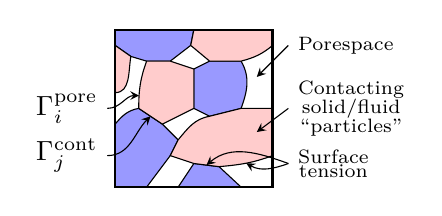
\begin{tikzpicture}[>=stealth,scale=2]
  \coordinate (A) at (0.35,0.2);
  \coordinate (B) at (0.4,0.3);
  \coordinate (C) at (0.3,0.4);
  \coordinate (D) at (0.15,0.5);
  \coordinate (E) at (0.66,0.13);
  \coordinate (F) at (0.6,0.45);
  \coordinate (G) at (0.8,0.5);
  \coordinate (H) at (0.5,0.5);
  \coordinate (I) at (0.5,0.75);
  \coordinate (J) at (0.6,0.8);
  \coordinate (K) at (0.8,0.8);
  \coordinate (L) at (0.35,0.8);
  \coordinate (M) at (0.5,1);
  \coordinate (N) at (0,0.9);
  \coordinate (O) at (0.1,0.83);
  \coordinate (P) at (0.5,0.15);
  \coordinate (Q) at (0.48,0.9);
  \coordinate (R) at (0.2,0.8);
  
  % Region 1 particles 
  \draw[fill=blue!40] 
  (0,0) -- (0.2,0) -- (A) -- (B) -- (C) -- (D) to[out=190,in=50] (0,0.4) -- cycle %A
  (0.4,0) -- (P) -- (E) -- (0.8,0) -- cycle %B
  (F) -- (G) to[out=70,in=-60] (K) -- (J) -- (I) -- (H) -- cycle %C
  (M) -- (Q) -- (L) -- (R) -- (O) -- (N) -- (0,1) -- cycle %D
  ;

  % Region 2 particles
  \draw[fill=red!20]
  (0,0.6) to[out=0,in=-100] (O) -- (N) -- cycle %E
  (D) to[out=90,in=-110] coordinate[near start] (surf3) (R) -- (L) -- (I) -- (H) -- (C) -- (D) coordinate[midway] (surf4) %F
  (M) -- (Q) -- (J) -- (K) to[out=15,in=-140] (1,0.9) -- (1,1) -- cycle %G
  (1,0.2) to[out=-160,in=5] coordinate[midway] (surf1) (E) -- (P) coordinate[midway] (surf2) -- (A) -- (B) to[out=50,in=-170] (F) -- (G) -- (1,0.5) -- cycle %H
  ;

  \draw[thick] (0,0) rectangle (1,1);

  % Annotations
  \draw[<-] (0.9,0.7) -- (1.1,0.9) node[right,font=\scriptsize] {Porespace};
  \draw[<-] (0.9,0.35) -- (1.1,0.5) node[right,font=\scriptsize] {\shortstack{Contacting\\[-0.4em]solid/fluid\\[-0.4em]``particles''}};
  \draw[<-] (surf1) to[out=-30,in=-160] (1.1,0.15) node[right,font=\scriptsize] {\shortstack{Surface\\[-0.4em]tension}};
  \draw[<-] (surf2) to[out=40,in=160] (1.1,0.15); % extra arrow
  \draw[<-] (surf3) to[out=180,in=0] (-0.05,0.5) node[left] {$\Gamma_i^{\mathrm{pore}}$};
  \draw[<-] (surf4) to[out=-135,in=0] (-0.05,0.2) node[left] {$\Gamma_j^{\mathrm{cont}}$};
\end{tikzpicture}
%     %\includegraphics{sintering_rve.pdf}
%     \caption{Microstructure of porous particulate material with sintering particles in contact. The sintering body is subjected to Dirichlet and Neumann boundary conditions on the external boundary.}
%     \label{fig:micro}
% \end{figure}
% %-----------------------------------------------------------------------------


\subsection{Surface tension}

With porous microstructures comes high surface to bulk ratio and with that the modeling of surface energy is important
The ``surface tension'' along particle/particle and particle/pore interfaces (the latter denoted pore boundaries) is considered to be the sole ``driving force'' of the sintering process, and it is defined in terms of a ``surface tension force'' acting in the tangent plane of the surface.
In the simplest (and most common) case of isotropic surface tension, this traction is characterized by the constant surface-specific surface energy $\gamma_\surf$ in the current configuration as the single material parameter.
Although we adopt this simplified model below in the numerical results, it is possible to consider the more general situation of anisotropic ``surface stress'' that may also depend on the surface deformation via a suitable constitutive assumption, cf.\ \cite{Steinmann2008:boundaryenergies}.

We shall adopt the general expression for the surface energy
\begin{align}
  \hat{\ts\sigma} \cdot \hat{\diff}
\label{eq:surface_energy}
\end{align}
where
\begin{align}
  \hat{\diff} &\defeq \diff \cdot \hat{\ts I}
\\
  \hat{\ts I} &\defeq  \ts I - \ta n \outerp \ta n
\end{align}
Here, $\ta{n}$ is taken positive outwards from a convex surface.
More specifically, we consider the special case of isotropic surface tension $\hat{\ts\sigma} = \gamma_\surf \hat{\ts I}$, for the numerical examples.
In this case we obtain the familiar equivalent surface traction
\begin{equation}
    \ta{t}_\surf\defeq -\kappa\gamma_\surf\ta{n}
\label{eq:surface_traction_strong}
\end{equation}
where $\kappa\defeq\ta{n}\cdot\hat{\diff}$ is the curvature.

% As shown in, e.g.\ \textsc{\"Ohman et al.} \cite{Ohman2012a}, it is possible to represent the surface tension force by an equivalent surface traction, henceforth denoted $\ta{t}_\fluct$, acting on the surface (or interface).
% In the presently assumed case of isotropic surface tension, $\ta{t}_\fluct$ is directed in the normal direction to the surface and is given as
% %-----------------------------------------------------------------
% \begin{equation}
%     \ta{t}_\surf\defeq -\kappa\gamma_\surf\ta{n}
% \label{eq:surface_traction_strong}
% \end{equation}
% %------------------------------------------------------------------
% where $\kappa\defeq\ta{n}\cdot\hat{\diff}$ is the curvature.



%The smooth space-curved surface segment $\Gamma$, as shown in \figref{fig:surfacestress}, is considered as a ``thin shell'' acted upon by the tractions $\ta{t}^+$ and $\ta{t}^-$ on the upper and lower sides.
%These tractions are part of the final solution in the case $\Gamma$ is the contact interface of two bodies (solid or fluid) with different material properties.
%When $\Gamma$ is an outer surface, then $\ta{t}^+$ represents a prescribed loading (or reaction from prescribed displacement), whereas $-\ta{t}^-$ is the traction acting on the material just below the surface.
%In addition, the ``surface tension force'' $\hat{\ta t}$ acts in the tangent plane of the thin shell.
%Equilibrium is expressed as
%%-----------------------------------------------------------------
%\begin{equation}
%    \int_{\Gamma} \left[\ta{t}^+ + \ta{t}^-\right] \dif a = \int_{\partial\Gamma} \hat{\ta t} \dif l = \ta{0}
%\label{eq101KR}
%\end{equation}
%%------------------------------------------------------------------
%Upon introducing the ``surface stress'' tensor $\hat{\ts\sigma}$ (with components only in the tangent plane), such that $\hat{\ta t}=\hat{\ts\sigma}\cdot\ta{m}$ and $\hat{\ts\sigma}\cdot\ta{n}=\ta{0}$, we may use the surface divergence theorem for a smooth surface segment to rephrase the curve integral in \eqref{eq101KR} as
%%-----------------------------------------------------------------
%\begin{equation}
%    \int_{\partial\Gamma} \hat{\ts\sigma}\cdot\ta{m} \dif l = \int_{\Gamma} \hat{\ts\sigma}\cdot\hat{\diff} \dif a + \int_{\Gamma} \kappa\hat{\ts\sigma}\cdot\ta{n} \dif a = \int_{\Gamma} \hat{\ts\sigma}\cdot\hat{\diff} \dif a
%\label{eq102KR}
%\end{equation}
%%------------------------------------------------------------------
%Here, $\hat\diff \defeq \diff - \ta{n}\nabla_n$ is the surface gradient operator and $\kappa\defeq\ta{n}\cdot\hat{\diff}$ is the curvature and $\ta{n}\defeq\ta{n}^+$ is taken positive outwards from a convex surfaceCombining \eqref{eq101KR} and \eqref{eq102KR} and localizing the result for any arbitrary choice of $\Gamma$, we obtain the strong format of traction equilibrium as follows:
%%-----------------------------------------------------------------
%\begin{equation}
%    \ta{t}^+ + \ta{t}^- + \ta{t}_\surf = \ta{0} \quad \mbox{on} \,\, \Gamma \quad \mbox{with } \ta{t}_\surf \defeq \hat{\ts\sigma}\cdot\hat{\diff}
%\label{eq103KR}
%\end{equation}
%%------------------------------------------------------------------
%where $\ta{t}_\surf$ is the ``surface tension traction''. Since it can be shown that $\ta{t}_\surf$ will depend on the (local) curvature, it is well-defined only when $\Gamma$ is sufficiently smooth
%
%Special case: Isotropic surface tension:
%
%Consider the special case that the surface tension is isotropic and homogeneous in the spatial format, i.e. $\hat{\ts\sigma}=\gamma_\surf\hat{\ts I}$, where $\gamma_\surf$ is a constant parameter and $\hat{\ts I} \defeq \ts{I} - \ta{n}\outerp\ta{n}$ is the surface identity tensor. Using the identity $\hat{\ts I}\cdot\hat{\diff}=-\kappa\ta{n}$, we then obtain
%%-----------------------------------------------------------------
%\begin{equation}
%    \sum_i \gamma_{\surf,i}\ta{m}_i = \ta{0} \quad \mbox{on} \,\, \mathcal{C}
%\label{eq104aKR}
%\end{equation}
%%------------------------------------------------------------------

\subsection{Balance equations - Strong and weak formats}

In the absence of acceleration, the balance equations for the quasi-static motion of the assembly of viscoplastic particles can be established in the spatial setting as follows:
%-----------------------------------------------------------------
\begin{subequations}\label{eq:strong_form}
\begin{align}
    -\ts{\sigma}\cdot\diff & = \ts{0} \quad \mbox{ in }\,\Omega^\particle_i\quad i = 1,2,...
\label{eq:strong_form_v}
\\
    \ta{v}\cdot\diff & = 0 \quad \mbox{ in }\,\Omega^\particle_i
\label{eq:strong_form_p}
\end{align}
\end{subequations}
%------------------------------------------------------------------
where $\ts{\sigma}(\ts{d})=\ts{\sigma}_\dev(\ts{d}_\dev)-p\ts{I}$ is the total Cauchy stress, $p$ is the pressure (Lagrangian multiplier corresponding to the incompressibility constraint), and
where $\diff$ denotes the spatial gradient.

% In order to establish the weak format of \eqref{eq:weak_form} for a sintering body, we henceforth assume (for simplicity) that the surface tension along the contact surfaces $\Gamma^\contact$ can be ignored; hence, the internal boundary of the domain $\Omega^\particle$ occupied by the particle assembly is $\Gamma^\pore$.
% It then appears that the space-variational forms of \eqref{eq:weak_form} read:

Referring to \figref{fig:micro}, we consider an arbitrarily chosen collection of particles in contact (inside $\Omega$)that constitutes the ``solid particle skeleton''.
Each particle domain $\Omega_i^\particle$ has part of its boundary associated with the pore surface $\Gamma_i^\pore$.
In addition, two particles are in contact across the surface $\Gamma_j^\contact$; however, we assume henceforth (for simplicity) that the surface tension along the contact surfaces can be ignored. We also introduce the notation $\Omega^\particle \defeq\cup_i\Omega_i^\particle$ and $\Gamma^\pore \defeq \cup_i\Gamma^\pore_i$.
%These surfaces, that are internal to the microstructure, are collectively denoted $\Gamma^\internal=\Gamma^\pore\cup\Gamma^\contact$.
The weak form of \eqref{eq:strong_form} then reads:
%-----------------------------------------------------------------
\begin{subequations}\label{eq:weak_form}
\begin{align}
    \int_{\Omega^\particle} \ts{\sigma}\dprod[\delta \ta v\outerp\diff] \dif v
    & =
    -\int_{\Gamma^\pore} \hat{\ts\sigma} \dprod [\delta\ta{v}\outerp\hat{\diff}] \dif a
\label{eq:weak_form_v} \\
    \int_{\Omega^\particle} \left[\ta{v}\cdot\diff\right] \delta p \dif v
    & =  0
\label{eq:weak_form_p}
\end{align}
\end{subequations}
%------------------------------------------------------------------
for suitable test functions $\delta\ta{v}$ and $\delta p$ that satisfy the appropriate regularity requirements (not further elaborated in this paper).

\textbf{Remark}: In the special case of isotropic surface tension (not necessarily homogeneous), the operational format of \eqref{eq:weak_form_v} is obtained by using the more explicit expression for the integral that represents ``surface tension loading'':
%-----------------------------------------------------------------
\begin{equation}
    \int_{\Gamma^\pore} \hat{\ts\sigma} \dprod [\delta\ta{v}\outerp\hat{\diff}] \dif a =
    \int_{\Gamma^\pore} \gamma_\surf\left[\delta\ta{v}\cdot\hat{\diff}\right] \dif a
\label{eq:surface_traction_weak}
\end{equation}
%------------------------------------------------------------------
where the surface divergence theorem was used for any smooth pore surface segment $\Gamma^\pore_i$. $\Box$

\section{Macro problem}
As shown in \textsc{\"Ohman et al.} \cite{Ohman2012b}, the macroscale problem can be put in the abstract form as follows: Find $(\bar{\ta v},\bar p) \in\bar{\set V}\times\bar{\set{P}}$ that solve
%----------------------------------------------------------------------------
\begin{subequations}\label{eq:macro}
\begin{alignat}{3}
 &\bar a\{\bar{\ta v},\bar p; \delta\bar{\ta v}\} + \bar b\{\bar p, \delta\bar{\ta v}\} &&= 0   &&\quad \forall\; \delta\bar{\ta v} \in \bar{\set{V}}^0
 \label{eq:macro_v}\\
 &\bar b\{\delta\bar p, \bar{\ta v}\} + \bar c\{\bar{\ta v}, \bar p; \delta\bar p\} &&= 0   &&\quad \forall\; \delta\bar p \in \bar{\set{P}}
 \label{eq:macro_p}
\end{alignat}
\end{subequations}
%----------------------------------------------------------------------------
where the pertinent variational forms are given as
%----------------------------------------------------------------------------
\begin{align}
 \bar a\{\bar{\ta v},\bar p; \delta\bar{\ta v}\} &\defeq \phantom{-}\int_\Omega \bar{\ts\sigma}_\dev\{\left[\bar{\ta v}\outerp \diff\right]^\sym_\dev,\bar p\}\dprod \left[\delta\bar{\ta v}\outerp \diff\right]^\sym_\dev \dif v
 \label{eq:macro_a}\\
 \bar b\{\bar p, \delta\bar{\ta v}\}             &\defeq -\int_\Omega \bar p\left[\delta\bar{\ta v}\cdot\diff\right]\dif v
 \label{eq:macro_b}\\
 \bar c\{\bar{\ta v}, \bar p; \delta\bar p\}     &\defeq \phantom{-}\int_\Omega \bar{e}\{\left[\bar{\ta v}\outerp \diff\right]^\sym_\dev,\bar p\}\delta\bar p\dif v
 \label{eq:macro_c}
 %\bar l\{\delta\bar {\ta v}\}               &\defeq \int_{\Gamma^\external_\Neumann} \bar{\ta t}_\prescribed\cdot \delta\bar{\ta v} \dif a
 %\label{eq:macro_l}
\end{align}
%----------------------------------------------------------------------------
The formulation in \eqref{eq:macro} allows for seamless transition from macroscopic compressible to incompressible by letting $\bar{c} \to 0$.
%In order to motivate the boundary term \eqref{eq412d}, we have assumed sufficient smoothness of the prescribed traction $\bar{\ta t}_\prescribed$.
Newton iterations for solving the system \eqref{eq:macro} employ the algorithmic tangents
%----------------------------------------------------------------------------
\begin{subequations}\label{eq:macro_sensitivity}
\begin{align}
 \dif \bar{\ts\sigma}_\dev &= \bar{\tf E}_\ded \dprod \dif\bar{\ts d}_\dev + \bar{\ts E}_\dep \dif\bar{p}
 \label{eq:macro_sensitivity_s} \\
 \dif \bar{e} &= \bar{\ts C}_\ded \dprod \dif \bar{\ts d}_\dev + \bar{C}_\dep \dif\bar{p}
 \label{eq:macro_sensitivity_e}
\end{align}
\end{subequations}
%-----------------------------------------------------------------------------
taken with respect to $\bar{\ts d}_\dev \defeq [\bar{\ta v}\outerp\diff]^\sym_\dev$ and $\bar p$, such that the increments $\Delta\bar{\ta v}$ and $\Delta\bar{p}$ are obtained from the macroscale tangent problem
%----------------------------------------------------------------------------
\begin{subequations}\label{eq:macro_tangent_problem}
\begin{alignat}{3}
  \bar{a}'_\derv\{\bullet; \delta\bar{\ta v},\Delta\bar{\ta v}\} + \bar{a}'_\dep\{\bullet; \delta\bar{\ta v},\Delta\bar{p}\} + \bar{b}\{\Delta\bar p, \delta\bar{\ta v}\}
  &= - \bar{a}\{\bullet; \delta\bar{\ta v}\} - \bar{b}\{\bullet, \delta\bar{\ta v}\}
  &\;\;&\forall\; \delta\bar{\ta v} \in \bar{\set{V}}^0
\label{eq:macro_tangent_problem_v}
\\
  \bar{b}\{\delta\bar p, \Delta\bar{\ta v}\} + \bar{c}'_\derv\{\bullet; \delta\bar{p}, \Delta\bar{ \ta v}\} + \bar{c}'_\dep\{\bullet; \delta\bar{p},\Delta\bar{p}\}
  &= -\bar{b}\{\delta\bar{p},\bullet\} - \bar{c}\{\bullet;\delta\bar{p}\}
  &\;\;&\forall\; \delta\bar{p} \in \bar{\set{P}}
\label{eq:macro_tangent_problem_p}
\end{alignat}
\end{subequations}
%----------------------------------------------------------------------------
where
%----------------------------------------------------------------------------
\begin{align}
 \bar{a}'_\derv\{\bullet; \delta\bar{\ta v},\Delta\bar{\ta v}\} &= \int_\Omega \left[\delta\bar{\ta v}\outerp\diff\right]^\sym_\dev \dprod \bar{\tf{E}}_\ded \dprod \left[\Delta\bar{\ta v}\outerp\diff\right]^\sym_\dev \dif v
 \label{eq:macro_av}\\
 \bar{a}'_\dep\{\bullet; \delta\bar{\ta v},\Delta\bar{p}\}     &= \int_\Omega \left[\delta\bar{\ta v}\outerp\diff\right]^\sym_\dev \dprod \bar{\ts E}_\dep \,\Delta\bar{p} \dif v
 \label{eq:macro_ap}\\
 \bar{c}'_\derv\{\bullet; \delta\bar{p}, \Delta\bar{ \ta v}\}   &= \int_\Omega \delta\bar{p} \,\bar{\ts C}_\ded \dprod \left[\Delta\bar{\ta v}\outerp\diff\right]^\sym_\dev \dif v
 \label{eq:macro_cv}\\
 \bar{c}'_\dep\{\bullet; \delta\bar{p},\Delta\bar{p}\}         &= \int_\Omega \delta\bar{p} \,\bar{C}_\dep \Delta\bar p\dif v.
 \label{eq:macro_cp}
\end{align}

\section{RVE problem}

\subsection{Preliminaries}
The macroscopic stress and rate of deformation gradient are split as
\begin{alignat}{3}
    &\bar{\ts d} = \bar{\ts d}_\dev + \frac{1}{3}\bar{e} \ts I
    &\;\;&\text{where}\;\; \bar{e} \defeq \bar{\ts d}\dprod \ts I,&\;\;& \bar{\ts d}_\dev \defeq \bar{\ts d} - \frac13\bar{e}\ts I \\
    &\bar{\ts\sigma} = \bar{\ts\sigma}_\dev - \bar{p} \ts I
    &\;\;&\text{where}\;\; \bar{p} \defeq -\frac13 \bar{\ts\sigma}\dprod \ts I,&\;\;& \bar{\ts\sigma}_\dev \defeq \bar{\ts\sigma} + \bar{p} \ts I
\end{alignat}
The deviatoric tensors can be expressed in a orthonormal base such that
\begin{subequations}
\begin{gather}
 \bar{\ts\sigma}_\dev = \sum_{i=1}^{n_{\mathrm{b}}} \bar{\sigma}_{\dev,i} \ts E_i,\quad \bar{\ts\sigma}_\dev \dprod \ts E_i = \bar{\sigma}_{\dev,i}
\label{eq:sigma_base} \\
 \bar{\ts d}_\dev = \sum_{i=1}^{n_{\mathrm{b}}} \bar{d}_{\dev,i} \ts E_i,\quad \bar{\ts d}_\dev \dprod \ts E_i = \bar{d}_{\dev,i}
\label{eq:d_base}
\end{gather}
\end{subequations}
where examples of base dyads are listed in Appendix \ref{sec:base_dyads}.

\subsection{RVE potential}

In order to show the Neumann-type boundary condition we shall first revisit the Dirichlet type boundary condition shown in \cite{Ohman2012b} but expressed as a minimization problem.
The subscale fluid is still subject to incompressibility constraint
\begin{gather}
 \diff \cdot \ta v = 0
\end{gather}
and the choice of homogenization of the deviatoric strain rate
\begin{align}
 \bar{\ts d}_\dev = \volume\int_{\Gamma_\Box} [\ta v \outerp \ta n] \dif A
\end{align}
% In the Dirichlet type boundary condition introduced in \cite{Ohman_etal2012b} the velocity on the boundary was controlled by the prolongated macroscopic deviatoric gradient, $\bar{\ts d}_\dev$, but now we introduce an additional constraint
% \begin{gather}
%  \volume \int_{\Gamma_\Box}[\ta v\outerp\ta n]_\dev \dif A = \bar{\ts d}_\dev
% \end{gather}
which leads to the suitable RVE-potential
\begin{multline}
 \Lambda_\Box(\bar{\ts d}_\dev, \bar{p}; \ta v, p, \ta t, \bar{e}) \defeq
\\
     \Lambda_\Box^\particle(\bar{\ts d}_\dev, \bar{p}; \ta v, p)
  + \bar{p}\; \bar{e}
  + \volume \int_{\Gamma_\Box^+} \ta t \cdot \jump{[\bar{\ts d}_\dev + \frac13\bar{e} \ts I]\cdot[\ta x - \bar{\ta x}] - \ta v}\dif A
\end{multline}
\begin{align}
 \Lambda_\Box^\particle(\bar{\ts d}_\dev, \bar{p}; \ta v, p) \defeq  \volume\int_{\Omega_\Box^\particle} [\Psi(\ta v\outerp\diff) - p\;[\ta v\cdot\diff]] \dif V
   + \volume\int_{\Gamma_\Box^\pore} \hat{\ts\sigma}_\dev\dprod[\ta v\outerp\hat{\diff}]\dif A.
\end{align}
Here we introduced $\Gamma_\Box^+$ and the jump $\jump{\bullet} \defeq \bullet^+ - \bullet^-$, where $+$ and $-$ represents the opposing sides on an cubic RVE.

%%%%%%%%%%%%%%%%%%%%%%%%%%%%%%%%%%%%%%%%%%%%%%%%%%%%%%%%%%%%%%%%%%%%%%%%%%%%%%%%%%%%%%%%%%%%%%%%%%%%%%%%%%%%%%%%%%%%%%%%
\subsubsection{Dirichlet boundary condition}
We can express the Dirichlet boundary condition using the same RVE-potential
\begin{align}
\label{eq:dirichlet_potential}
 \Psi^\Dirichlet_\Box(\bar{\ts d}_\dev, \bar{p} ) \defeq
    \inf_{\substack{ \ta v \in \set V_\Box^\Dirichlet \\ \bar{e} \in \set{R} }} \;
    \sup_{\substack{ p\in \set P_\Box \\ \ta t \in \set{T}_\Box }}
    \Lambda_\Box(\bar{\ts d}_\dev, \bar{p}; \ta v, p, \ta t, \bar{e})
\end{align}
where
\begin{align}
 \set{V}_\Box^\Dirichlet &= \{ \ta v \in \set{V}_\Box : \exists\; (\hat{\ts d}_\dev,\bar{e}) \in \set{R}^{3\times 3}_\dev \times \set{R} : \ta v = \hat{\ts d}_\dev\cdot[\ta x - \bar{\ta x}] + \bar{e}\; \ta x_\mean \text{ on }\Gamma_\Box \} \\
 \ta x_\mean        &\defeq \frac13 [\ta x - \bar{\ta x}].
\end{align}
Simplifying \eqref{eq:dirichlet_potential} we obtain
\begin{align}
\nonumber
 \Psi^\Dirichlet_\Box(\bar{\ts d}_\dev, \bar{p} ) &=
    \inf_{\substack{ \ta v^\fluct \in \set V_\Box^0 \\ \bar{e} \in \set R \\ \hat{\ts d}_\dev \in \set{R}_\dev^{3\times 3} }} \;
    \sup_{\substack{ p\in \set P_\Box \\ \bar{\ts\sigma}_\dev \in \set{R}_\dev^{3\times 3} }}
    \Lambda_\Box(\bar{\ts d}_\dev, \bar{p}; \hat{\ts d}_\dev \cdot [\ta x - \bar{\ta x}] + \bar{e}\; \ta x_\mean + \ta v^\fluct, p, \ta t, \bar{e})
\intertext{ \{ $\hat{\ts d}_\dev = \bar{\ts d}_\dev$ only possible minimum due to $\sup\;\bar{\ts\sigma}_\dev$ \} }
  &=
    \inf_{\substack{ \ta v^\fluct \in \set V_\Box^0 \\ \bar{e} \in \set R }} \;
    \sup_{\substack{ p\in \set P_\Box }}
    \Lambda_\Box(\bar{\ts d}_\dev, \bar{p}; \bar{\ts d}_\dev \cdot [\ta x - \bar{\ta x}] + \bar{e}\; \ta x_\mean + \ta v^\fluct, p, \ta t, \bar{e})
\\
  &=
    \inf_{\substack{ \ta v^\fluct \in \set V_\Box^0 \\ \bar{e} \in \set R }} \;
    \sup_{\substack{ p\in \set P_\Box }}
    \Lambda_\Box^\particle(\bar{\ts d}_\dev, \bar{p}; \bar{\ts d}_\dev \cdot [\ta x - \bar{\ta x}] + \bar{e}\; \ta x_\mean + \ta v^\fluct, p) + \bar{p}\;\bar{e}
\end{align}
where
\begin{align}
 \set{V}_\Box^0 &= \{ \ta v^\fluct \in \set{V}_\Box : \ta v^\fluct = \ta 0 \text{ on }\Gamma_\Box \}.
\end{align}

% We can express the RVE-potential as
% \begin{multline}
%  \Lambda_\Box \equiv \Lambda_\Box^\Dirichlet(\bar{\ts d}_\dev, \bar{p}; \ta v^\fluct, p, \bar{e}) \defeq 
%   \volume \int_{\Omega_\Box^\particle} \Psi(\bar{\ts d}_\dev + \ta v^\fluct \outerp \diff) - p [\ta v^\fluct \cdot \diff] \dif V \\ 
%  +  \bar{e} [\bar{p} - \volume \int_{\Omega_\Box^\particle} p \dif V]
%  + \volume \int_{\Gamma_\Box^\pore} \hat{\ts\sigma}\dprod [\bar{\ts d}_\dev \cdot \ta x + \bar{e}\;\ta x_\mean + \ta v^\fluct]\outerp\hat{\diff}]\dif A
% \end{multline}
%and
Introducing the stationarity condition we obtain the weak form for the Dirichlet type boundary condition: Find $(\ta v^\fluct, p, \bar{e}) \in \set{V}_\Box^0\times\set{P}_\Box\times\set{R}$ such that
% \begin{align}
%  \Lambda^{\Dirichlet\prime}_{\Box,\ta v^\fluct} (\bar{\ta d}_\dev, \bar{p};\ta v^\fluct, p, \bar{e}; \delta\ta v^\fluct) = 0 \forall \delta v^\fluct \in \set{V}_\Box^0
% \end{align}
\begin{alignat}{4}
 &a_\Box(\bar{\ts d}_\dev\cdot[\ta x-\bar{\ta x}] + \ta v^\fluct; \delta\ta v^\fluct) + b_\Box(p,\delta\ta v^\fluct) &&= l_\Box(\delta\ta v^\fluct)
&\quad &\forall\;\delta\ta v^\fluct &&\in \set{V}_\Box^0
\\
 &b_\Box(\delta p, \bar{e}\;\ta x_\mean + \ta v^\fluct) &&= 0
&\quad &\forall\;\delta p&&\in\set{P}_\Box
\\
 &b_\Box(p, \ta x_\mean) \delta\bar{e} &&= [l_\Box(\ta x_\mean) - \bar p]\delta\bar{e} 
&\quad &\forall\;\delta\bar{e}&&\in\set{R}
\end{alignat}
where the abstract forms are as given in \eqref{eq:rve_a}, \eqref{eq:rve_b}, \eqref{eq:rve_l}.
% \begin{alignat}{2}
%  a_\Box(\ta v; \delta\ta v) &\defeq \phantom{-}\volume \int_{\Omega_\Box^\particle} \ts\sigma_\dev\dprod[\delta\ta v\outerp\diff] \dif V  \\
%  b_\Box(p, \ta v)           &\defeq -\volume \int_{\Omega_\Box^\particle} p\;[\ta v\cdot\diff] \dif V   \\
%  l_\Box(\delta\ta v)        &\defeq -\volume \int_{\Gamma_\Box^\pore}\hat{\ts\sigma}\dprod[\delta\ta v \outerp\hat{\diff}] \dif A
% \end{alignat}

The macroscopic response is obtained from
\begin{align}
 \bar{\ts\sigma}_\dev &= \pd{\Psi_\Box^\Dirichlet}{\bar{\ts d}_\dev} = \volume \left[
    \int_{\Omega_\Box^\particle} \bar{\ts\sigma}_\dev \dif V + 
    \int_{\Gamma_\Box^\pore} [\hat{\ts\sigma}\dprod[\ta x \outerp \hat{\diff}]]_\dev \dif A \right] =
\nonumber\\
    &= \volume \int_{\Gamma_\Box} [\ta t \outerp \ta x] \dif A + \bar{p}\;\ts I
\\
 \bar{e} &= \pd{\Psi_\Box^\Dirichlet}{\bar{p}} = \bar{e} \quad \text{(by construction)}
\end{align}


%%%%%%%%%%%%%%%%%%%%%%%%%%%%%%%%%%%%%%%%%%%%%%%%%%%%%%%%%%%%%%%%%%%%%%%%%%%%%%%%%%%%%%%%%%%%%%%%%%%%%%%%%%%%%%%%%%%%%%%%
\subsubsection{Neumann boundary condition}
We can obtain the Neumann boundary condition by restricting the space for $\ta t$:
\begin{align}
 \Psi^\Neumann_\Box(\bar{\ts d}_\dev, \bar{p} ) &\defeq
    \inf_{\substack{\ta v \in \set V_\Box \\ \bar{e} \in R}} \;
    \sup_{\substack{p\in \set P_\Box \\ \ta t \in \set T_\Box^\Neumann}} \Lambda_\Box(\bar{\ts d}_\dev, \bar p; \ta v, p, \ta t, \bar{e})
\label{eq:neumann_potential}
\end{align}
where
\begin{align}
 \set T_\Box^\Neumann = \{ \ta t : \exists\; (\bar{\ts\sigma}_\dev, \hat{p}) \in \set{R}^{3\times 3}_\dev \times \set{R} : \ta t = \bar{\ts\sigma}_\dev\cdot\ta n - \hat{p}\;\ta n \}
\end{align}
Simplifying \eqref{eq:neumann_potential} we obtain
\begin{align}
 \Psi^\Neumann_\Box(\bar{\ts d}_\dev, \bar{p} ) &\defeq
    \inf_{\substack{\ta v \in \set V_\Box \\ \bar{e} \in R}} \;
    \sup_{\substack{p\in \set P_\Box \\ \bar{\ts\sigma}_\dev\in \set{R}_\dev^{3\times 3} \\ \hat{p}\in \set{R} }} \Lambda_\Box(\bar{\ts d}_\dev, \bar p; \ta v, p, \bar{\ts\sigma}_\dev\cdot\ta n - \hat{p}\;\ta n, \bar{e})
\intertext{ \{ $\hat{p} = \bar{p}$ only possible minimum due to $\inf\;\bar{e}$ \} }
    &= 
    \inf_{\ta v \in \set V_\Box} \;
    \sup_{\substack{p\in \set P_\Box \\ \bar{\ts\sigma}_\dev\in \set{R}_\dev^{3\times 3}}}
    \Lambda_\Box(\bar{\ts d}_\dev, \bar p; \ta v, p, \bar{\ts\sigma}_\dev\cdot\ta n, 0)
\\
    &=
    \inf_{\ta v \in \set V_\Box} \;
    \sup_{\substack{p\in \set P_\Box \\ \bar{\ts\sigma}_\dev\in \set{R}_\dev^{3\times 3}}}
    \!\!\Lambda_\Box^\particle(\bar{\ts d}_\dev, \bar p; \ta v, p) + 
    \left[\bar{\ts d}_\dev - \volume\int_{\Gamma_\Box} [\ta v\outerp\ta n] \dif A\right]\dprod \bar{\ts\sigma}_\dev.
\end{align}

Stationarity gives us the weak form: Find $(\ta v, p, \bar{\ts\sigma}_\dev) \in \set{V}_\Box \times \set{P}_\Box \times \set{R}_\dev^{3\times 3}$ such that
\begin{subequations}\label{eq:rve_neumann}
\begin{alignat}{4}
 &a_\Box(\ta v, \delta\ta v) + b_\Box(p,\delta\ta v) + c_\Box(\bar{\ts\sigma}_\dev, \delta\ta v) &&= f_\Box(\bar{p},\delta\ta v) + l_\Box(\delta\ta v)
&\;\;& \forall\; \delta\bar{\ta v} &&\in \set{V}_\Box
 \\
 &b_\Box(\delta p, \ta v) &&= 0
&& \forall\; \delta p &&\in \set{P}_\Box
 \\
 &c_\Box(\delta\bar{\ts\sigma}_\dev, \ta v) &&= -\bar{\ts d}_\dev \dprod \delta\bar{\ts\sigma}_\dev
&& \forall\; \delta\bar{\ts\sigma}_\dev &&\in \set{R}^{3 \times 3}_\dev
\label{eq:rve_neumann_sigma}
\end{alignat}
\end{subequations}
where
\begin{alignat}{2}
 \label{eq:rve_a}
 a_\Box(\ta v, \delta\ta v)          &\defeq \phantom{-} \volume \int_{\Omega_\Box^\particle} \ts\sigma_\dev \dprod [\delta\ta v\outerp\diff] \dif V \\
 \label{eq:rve_b}
 b_\Box(p, \ta v)                    &\defeq -\volume \int_{\Omega_\Box^\particle} p\;[\ta v\cdot\diff] \dif A \\
 \label{eq:rve_c}
 c_\Box(\bar{\ts\sigma}_\dev, \ta v) &\defeq -\volume \int_{\Gamma_\Box} [\ta v\outerp\ta n]_\dev \dif A \dprod \bar{\ts\sigma}_\dev\\
 \label{eq:rve_f}
 f_\Box(\bar{p},\delta\ta v)         &\defeq -\volume \int_{\Gamma_\Box} [\delta\ta v\cdot\ta n] \dif A\; \bar{p} \\
 \label{eq:rve_l}
 l_\Box(\delta\ta v)                 &\defeq -\volume \int_{\Gamma_\Box^\pore} \hat{\ts\sigma} \dprod [\delta\ta v\outerp\hat{\diff}] \dif A
\end{alignat}
% With \eqref{eq:rve_neumann} we solve for $\bar{\ts\sigma}_\dev$ directly while $\bar{e}$ is obtained through post-processing
% \begin{align}
%  \bar{e} = \volume\int_{\Gamma_\Box} [\ta v \cdot \ta n]\dif A.
% \end{align}
The macroscopic responses are defined from the potential as
\begin{align}
 \bar{\ts\sigma}_\dev &= \pd{\Psi^\Neumann}{\bar{\ts d}_\dev} = \pd{\Lambda_\Box}{\bar{\ts d}_\dev} = \bar{\ts\sigma}_\dev \quad\text{(by construction})
\\
 \bar{e} &= \pd{\Psi^\Neumann}{\bar{p}} = \pd{\Lambda_\Box}{\bar{p}} = \volume \int_{\Gamma_\Box} [\ta v \cdot \ta n] \dif A
\end{align}
%
\textbf{Remark:} When solving \eqref{eq:rve_neumann_sigma}, it is expanded in the deviatoric base and obtain the set of scalar equations to solve
\begin{alignat}{4}
 &c_\Box(\delta\bar{\sigma}_{\dev,i} \ts E_i, \ta v) &&= -\bar{d}_{\dev,i} \delta\bar{\sigma}_{\dev,i}.
&\quad\quad& \forall\; \delta\bar{\sigma}_{\dev,i} &&\in \set{R}
\end{alignat}
for $i = 1, \ldots, n_{\mathrm{b}}$.

%%%%%%%%%%%%%%%%%%%%%%%%%%%%%%%%%%%%%%%%%%%%%%%%%%%%%%%%%%%%%%%%%%%%%%%%%%%%%%%%%%%%%%%%%%%%%%%%%%%%%%%%%%%%%%%%%%%%%%%%
\subsubsection{Periodic boundary condition}
We can express the periodic boundary condition using the same RVE-potential
\begin{align}
  \Psi^\Periodic_\Box(\bar{\ts d}_\dev, \bar{p} ) &\defeq
    \inf_{\substack{\ta v \in \set V_\Box \\ \bar{e} \in R}} \;
    \sup_{\substack{p\in \set P_\Box \\ \ta t \in \set T_\Box^\Periodic}} \Lambda_\Box(\bar{\ts d}_\dev, \bar p; \ta v, p, \ta t, \bar{e})
\label{eq:periodic_potential}
\end{align}
.............
\begin{align}
\label{eq:periodic_potential}
 \Psi^\Periodic_\Box(\bar{\ts d}_\dev, \bar{p} ) \defeq
    \inf_{\ta v \in \set V_\Box^\Periodic} \;
    \sup_{\substack{ p\in \set P_\Box \\ \bar{\ts\sigma}_\dev \in \set{R}_\dev^{3\times 3} }}
    \Lambda_\Box(\bar{\ts d}_\dev, \bar{p}; \ta v, p, \bar{\ts\sigma}_\dev)
\end{align}
where
\begin{align}
 \set{V}_\Box^\Periodic &= \{ \ta v \in \set{V}_\Box : \exists\; (\hat{\ts d}_\dev,\bar{e}) \in \set{R}^{3\times 3}_\dev \times \set{R} : \jump{\ta v} = \hat{\ts d}_\dev\cdot\jump{\ta x - \bar{\ta x}} + \bar{e}\; \jump{\ta x_\mean} \text{ on }\Gamma_\Box^+ \}.
\end{align}

Simplifying \eqref{eq:periodic_potential} we obtain
\begin{align}
\nonumber
 \Psi^\Periodic_\Box(\bar{\ts d}_\dev, \bar{p} ) &=
    \inf_{\substack{ \ta v^\fluct \in \set V_\Box^{0+} \\ \bar{e} \in \set R \\ \hat{\ts d}_\dev \in \set{R}_\dev^{3\times 3} }} \;
    \sup_{\substack{ p\in \set P_\Box \\ \bar{\ts\sigma}_\dev \in \set{R}_\dev^{3\times 3} }}
    \Lambda_\Box(\bar{\ts d}_\dev, \bar{p}; \hat{\ts d}_\dev \cdot [\ta x - \bar{\ta x}] + \bar{e}\; \ta x_\mean + \ta v^\fluct, p, \bar{\ts\sigma}_\dev)
\intertext{ \{ $\hat{\ts d}_\dev = \bar{\ts d}_\dev$ only possible minimum due to $\sup\;\bar{\ts\sigma}_\dev$ \} }
  &=
    \inf_{\substack{ \ta v^\fluct \in \set V_\Box^{0+} \\ \bar{e} \in \set R }} \;
    \sup_{\substack{ p\in \set P_\Box }}
    \Lambda_\Box(\bar{\ts d}_\dev, \bar{p}; \bar{\ts d}_\dev \cdot [\ta x - \bar{\ta x}] + \bar{e}\; \ta x_\mean + \ta v^\fluct, p, \bar{\ts\sigma}_\dev)
\end{align}
where
\begin{align}
 \set{V}_\Box^{0+} &= \{ \ta v^\fluct \in \set{V}_\Box : \jump{\ta v^\fluct} = \ta 0 \text{ on }\Gamma_\Box \}
\end{align}

Introducing the stationarity condition we obtain the weak form for the Periodic type boundary condition: Find $(\ta v^\fluct, p, \bar{e}) \in \set{V}_\Box^{0+}\times\set{P}_\Box\times\set{R}$ such that
\begin{alignat}{4}
 &a_\Box(\bar{\ts d}_\dev\cdot[\ta x-\bar{\ta x}] + \ta v^\fluct; \delta\ta v^\fluct) + b_\Box(p,\delta\ta v^\fluct) &&= l_\Box(\delta\ta v^\fluct)
&\quad &\forall\;\delta\ta v^\fluct &&\in \set{V}_\Box^{0+}
\\
 &b_\Box(\delta p, \bar{e}\;\ta x_\mean + \ta v^\fluct) &&= 0
&\quad &\forall\;\delta p&&\in\set{P}_\Box
\\
 &b_\Box(p, \ta x_\mean) \delta\bar{e} &&= [l_\Box(\ta x_\mean) - \bar p]\delta\bar{e} 
&\quad &\forall\;\delta\bar{e}&&\in\set{R}
\end{alignat}

\todo{Check sigma}
The macroscopic response is obtained from
\begin{align}
 \bar{\ts\sigma}_\dev &= \pd{\Psi_\Box^\Periodic}{\bar{\ts d}_\dev} = \volume \left[
    \int_{\Omega_\Box^\particle} \bar{\ts\sigma}_\dev ??????? \dif V + 
    \int_{\Gamma_\Box^\pore} [\hat{\ts\sigma}\dprod[\ta x \outerp \hat{\diff}]]_\dev ??????? \dif A 
\right]
 \\
 &= \volume \int_{\Gamma_\Box} [\ta t \outerp \ta x] \dif A + \bar{p} \ts I
% =
%\nonumber\\
%    &= \volume \int_{\Gamma_\Box} [\ta t \outerp \ta x] \dif A + \bar{p}\;\ts I
\\
 \bar{e} &= \pd{\Psi_\Box^\Periodic}{\bar{p}} = \bar{e} \quad \text{(by construction)}
\end{align}


\subsubsection{Bounds}
Hence, since 
\begin{align}
 \set{V}_\Box^\Dirichlet \subset \set{V}_\Box\\
 \set{T}_\Box^\Neumann \subset \set{T}_\Box
\end{align}
we have that
\begin{align}
 \Psi^\Dirichlet_\Box(\bar{\ts d}_\dev, \bar{p}) \geq \Psi^\Periodic(\bar{\ts d}_\dev, \bar {p}) \geq \Psi^\Neumann(\bar{\ts d}_\dev, \bar {p}).
\end{align}

For linear response we obtain
\begin{alignat}{4}
 &\Psi_\Box(\bar{\ts d}_\dev, 0) &&= \frac12 \bar{\ts d}_\dev \dprod \bar{\tf E}_{\ded} + \bar{\ts\sigma}_{\dev,0} \dprod \bar{\ts d}_\dev 
&\quad&\forall\;\bar{\ts d}_\dev &&\implies
 \bar{\tf E}_{\ded}^\Dirichlet \geq \bar{\tf E}_{\ded}^\Periodic \geq \bar{\tf E}_{\ded}^\Neumann
\\
 &\Psi_\Box(\ts 0, \bar{p}) &&= -\frac12 \bar{p}\;\bar{C}_{\dep}\;\bar{p} + \bar{e}_0\;\bar{p} 
&\quad&\forall\;\bar{p} &&\implies
 \bar{C}_\dep^\Dirichlet \leq \bar{C}_\dep^\Periodic \leq \bar{C}_\dep^\Neumann
\end{alignat}
for the tangents $\bar{\tf E}_\ded, \bar{C}_\dep$ which are defined in \eqref{eq:macro_tangents}.


%%%%%%%%%%%%%%%%%%%%%%%%%%%%%%%%%%%%%%%%%%%%%%%%%%%%%%%%%%%%%%%%%%%%%%%%%%%%%%%%%%%%%%%%%%%%%%%%%%%%%%%%%%%%%%%%%%%%%%%%
% \subsubsection{Weakly Periodic boundary condition}
% Maybe even do this? Generalize the Neumann and periodic boundary condition;
% \begin{align}
% \label{eq:dirichlet_potential}
%  \Psi^\Dirichlet_\Box(\bar{\ts d}_\dev, \bar{p} ) \defeq
%     \inf_{\ta v^\fluct \in \set V_\Box^\Dirichlet} \;
%     \sup_{\substack{ p\in \set P_\Box \\ \bar{\ts\sigma}_\dev \in \set{R}_\dev^{3\times 3} }}
%     \Lambda_\Box(\bar{\ts d}_\dev, \bar{p}; \bar{\ts d}_\dev \cdot [\ta x - \bar{\ta x}] + \bar{e} \ta x_\mean + \ta v^\fluct, p, \bar{\ts\sigma}_\dev)
% \end{align}
% where
% \begin{align}
%  \set{V}_\Box^\Dirichlet &= \{ \ta v \in \set{V}_\Box : \exists\; (\hat{\ts d}_\dev,\bar{e}) \in \set{R}^{3\times 3}_\dev \times \set{R} : \ta v = \hat{\ts d}_\dev\cdot[\ta x - \bar{\ta x}] + \bar{e}\; \ta x_\mean \text{ on }\Gamma_\Box \}
% \end{align}

%%%%%%%%%%%%%%%%%%%%%%%%%%%%%%%%%%%%%%%%%%%%%%%%%%%%%%%%%%%%%%%%%%%%%%%%%%%%%%%%%%%%%%%%%%%%%%%%%%%%%%%%%%%%%%%%%%%%%%%%%%%%%%%%%%%%%%%%%%%%%%%%%%%%%%%%%%%%%%
\subsection{Sensitivity analysis -- Neumann boundary condition}
In order to solve the macroscopic problem with Newtons method, we need to obtain the tangents
\begin{align}\label{eq:macro_tangents}
 \bar{\tf E}_\ded \defeq \pd{\bar{\ts\sigma}_\dev}{\bar{\ts d}_\dev}, \quad
 \bar{\ts E}_\dep \defeq \pd{\bar{\ts\sigma}_\dev}{\bar{p}}, \quad
 \bar{    C}_\dep \defeq \pd{\bar{e}}{\bar{p}}, \quad
 \bar{\ts C}_\ded \defeq \pd{\bar{e}}{\bar{\ts d}_\dev}
\end{align}
As before, we can express them in the deviatoric base
\begin{align}
 \bar{\ts C}_\ded \defeq \;&\pd{\bar{e}}{\bar{\ts d}_\dev} = \sum_{i=1}^{n_\mathrm{b}} \pd{\bar{e}}{\bar{d}_{\dev,i}} \ts E_i\\
 \bar{\ts E}_\dep \defeq \;&\pd{\bar{\ts\sigma}_\dev}{\bar{p}} = \sum_{i=1}^{n_\mathrm{b}} \pd{\bar{\sigma}_{\dev,i}}{\bar{p}} \ts E_i\\
 \bar{\tf E}_\ded \defeq \;&\pd{\bar{\ts\sigma}_\dev}{\bar{\ts d}_\dev} =  \sum_{i,j=1}^{n_\mathrm{b}} \pd{\bar{\sigma}_{\dev,i}}{\bar{d}_{\dev,j}} \ts E_i \outerp \ts E_j
\end{align}
where they can be determined from a sensitivity analysis such that
\begin{align}
 \bar{    C}_\dep &= \hat{\bar{e}}_{\dep}\\
 \bar{\ts C}_\ded &= \sum_{i=1}^{n_\mathrm{b}} \hat{\bar{e}}_{\ded}^{(i)}\;\ts E_i\\
 \bar{\ts E}_\dep &= \sum_{i=1}^{n_\mathrm{b}} \hat{\bar{\sigma}}_{\dev,i,\dep}\;\ts E_i\\
 \bar{\tf E}_\ded &= \sum_{i,j=1}^{n_\mathrm{b}} \hat{\bar{\sigma}}_{\dev,i,\ded}^{(j)}\;\ts E_i \outerp \ts E_j
\end{align}

Using the perturbations $\bar{d}_{\dev,k} + \dif\bar{d}_{\dev,k}$ and $\bar{p} + \dif\bar{p}$ in the linearized form at equilibrium we obtain
\begin{subequations}
\begin{alignat}{4}
 &(a_\Box)'(\ta v; \delta\ta v, \Delta\ta v) + b_\Box(\Delta p,\delta\ta v) + c_\Box(\Delta\bar{\sigma}_{\dev,i}\ts E_i,\delta\ta v) = f_\Box(\dif\bar{p},\delta\ta v)
&\;\;& \forall\; \delta\bar{\ta v} &&\in \set{V}_\Box
\\
 &b_\Box(\delta p, \Delta\ta v) = 0
&& \forall\; \delta p &&\in \set{P}_\Box
\\
 &c_\Box(\delta\bar{\sigma}_{\dev,i}\ts E_i,\Delta\ta v) = -\dif\bar{d}_{\dev,i} \; \delta\bar{\sigma}_{\dev,i}
&& \forall\; \delta\bar{\sigma}_{\dev,i} &&\in \set{R}
\end{alignat}
\end{subequations}
which must hold for any given $\dif\bar{d}_{\dev,i}$ and $\dif\bar{p}$. We thus consider the cases
\begin{enumerate}
 \item[1] $\dif\bar{d}_{\dev,k} = 1$, $\dif\bar{d}_{\dev,j} = 0$ for $j\neq k$ while $\dif\bar{p} = 0$: For $k = 1, \ldots, n_\mathrm{b}$, solve the sensitivities $\hat{\ta v}_\ded^{(k)}$, $\hat{p}_\ded^{(k)}$, $\hat{\bar{\sigma}}_{\dev,i,\ded}^{(k)}$ from the system 
\end{enumerate}
\begin{subequations}\label{eq:sensitivities_d}
\begin{alignat}{4}
 &(a_\Box)'(\ta v; \delta\ta v, \hat{\ta v}_\ded^{(k)}) + b_\Box(\hat{p}_\ded^{(k)},\delta\ta v) + c_\Box(\hat{\bar{\sigma}}_{\dev,i,\ded}^{(k)}\ts E_i,\delta\ta v) = 0
&\;\;& \forall\; \delta\bar{\ta v} &&\in \set{V}_\Box
\\
 &b_\Box(\delta p, \hat{\ta v}_\ded^{(k)}) = 0
&& \forall\; \delta p &&\in \set{P}_\Box
\\
 &c_\Box(\delta\bar{\sigma}_{\dev,i}\ts E_i,\hat{\ta v}_\ded^{(k)}) = -\delta_{ik} \; \delta\bar{\sigma}_{\dev,i}
&& \forall\; \delta\bar{\sigma}_{\dev,i} &&\in \set{R}
\end{alignat}
\end{subequations}
\begin{enumerate}
\item[2] $\dif\bar{p} = 1$ while $\dif\bar{d}_{\dev,k} = 0$: Solve the sensitivities $\hat{\ta v}_\dep$, $\hat{p}_\dep$, $\hat{\bar\sigma}_{\dev,i,\dep}$ from the system 
\end{enumerate}
\begin{subequations}\label{eq:sensitivities_p}
\begin{alignat}{4}
 &(a_\Box)'(\ta v; \delta\ta v, \hat{\ta v}_\dep) + b_\Box(\hat{p}_\dep,\delta\ta v) + c_\Box(\hat{\bar{\sigma}}_{\dev,i,\dep}\ts E_i,\delta\ta v) = f_\Box(1,\delta\ta v)
&\;\;& \forall\; \delta\bar{\ta v} &&\in \set{V}_\Box
\\
 &b_\Box(\delta p, \hat{\ta v}_\dep) = 0
&& \forall\; \delta p &&\in \set{P}_\Box
\\
 &c_\Box(\delta\bar{\sigma}_{\dev,i}\ts E_i,\hat{\ta v}_\dep) = 0
&& \forall\; \delta\bar{\sigma}_{\dev,i} &&\in \set{R}
\end{alignat}
\end{subequations}
The stresses, $\hat{\bar{\sigma}}_{\dev,i,\ded}^{(k)}$ and $\hat{\bar{\sigma}}_{\dev,i,\dep}$, are solved for directly, and the volumetric strain rates are post-processed as
\begin{align}
 \hat{\bar{e}}_{\ded}^{(k)} &= \volume\int_{\Gamma_\Box} [\hat{\ta v}_{\ded}^{(k)} \cdot \ta n]\dif A\\
 \hat{\bar{e}}_\dep &= \volume\int_{\Gamma_\Box} [\hat{\ta v}_\dep \cdot \ta n]\dif A 
\end{align}


%%%%%%%%%%%%%%%%%%%%%%%%%%%%%%%%%%%%%%%%%%%%%%%%%%%%%%%%%%%%%%%%%%%%%%%%%%%%%%%%%%%%%%%%%%%%%%%%%%%%%%%%%%%%%%%%%%%%%%%%%%%%%%%%%%%%%%%%%%%%%%%%%%%%%%%%%%%%%%
\section{Numerical examples}
\begin{itemize}
 \item Numerical comparison for free sintering with dirichlet and neumann b.c
 \item Numerical comparison for sheared sintering with dirichlet and neumann b.c
 \item Numerical comparison for FE2 with dirichlet and neumann b.c.
\end{itemize}


%%%%%%%%%%%%%%%%%%%%%%%%%%%%%%%%%%%%%%%%%%%%%%%%%%%%%%%%%%%%%%%%%%%%%%%%%%%%%%%%%%%%%%%%%%%%%%%%%%%%%%%%%%%%%%%%%%%%%%%%%%%%%%%%%%%%%%%%%%%%%%%%%%%%%%%%%%%%%%
\section{Discussion}

%%%%%%%%%%%%%%%%%%%%%%%%%%%%%%%%%%%%%%%%%%%%%%%%%%%%%%%%%%%%%%%%%%%%%%%%%%%%%%%%%%%%%%%%%%%%%%%%%%%%%%%%%%%%%%%%%%%%%%%%%%%%%%%%%%%%%%%%%%%%%%%%%%%%%%%%%%%%%%
\appendix
\section{Base dyadics in for deviatoric tensors}
\label{sec:base_dyads}


The orthonormal base for deviatoric (but generally unsymmetric) $\ts E_i$ can be chosen in a cartesian basis, in 2D, as
\begin{align}
 \ts E_1 = \frac{1}{\sqrt{2}}\begin{bmatrix} 1 & 0\\ 0 & -1\end{bmatrix}
\quad \ts E_2 = \begin{bmatrix} 0 & 1\\ 0 & 0\end{bmatrix}
\quad \ts E_3 = \begin{bmatrix} 0 & 0\\ 1 & 0\end{bmatrix}
\end{align}
and in 3D, as
\begin{equation}
\begin{gathered}
 \ts E_1 = \frac{1}{\sqrt{6}}\left[\begin{smallmatrix} 2 & 0 & 0\\ 0 & -1 & 0\\ 0 & 0 & -1\end{smallmatrix}\right],\;
 \ts E_2 = \left[\begin{smallmatrix} 0 & 0 & 0\\ 0 & 1 & 0 \\ 0 & 0 & -1\end{smallmatrix}\right],\;
 \ts E_3 = \left[\begin{smallmatrix} 0 & 1 & 0\\ 0 & 0 & 0 \\ 0 & 0 & 0\end{smallmatrix}\right],\;
 \ldots,\;
 \ts E_8 = \left[\begin{smallmatrix} 0 & 0 & 0\\ 0 & 0 & 0 \\ 0 & 1 & 0\end{smallmatrix}\right].
\end{gathered}
\end{equation}

\end{document}



\subsection{Incompressible viscous flow of the Stokes' type}

We shall adopt a model for the subscale deformation within the solid particles undergoing the time-dependent sintering process.
The model is simplified in the sense that elastic deformation is neglected a priori.
It is then possible to consider a viscoplastic (fluid-like) material with intrinsic incompressibility (within the particles).
Such incompressibility is expressed as $\ta{v}\cdot\ts{\nabla}=0$ and, hence, $\ts{d}_\dev=\ts{d}\defeq[\ta v\outerp\diff]^\sym$.
An isotropic and associated viscoplastic flow rule of the classical Perzyna type is proposed as follows:
%-----------------------------------------------------------------
\begin{equation}
    \ts{d}_\dev = \frac{1}{2\mu}\ts{\sigma}_\dev + \ts{d}_\dev^\pl(\ts{\sigma}_\dev), \quad
    \ts{d}_\dev^\pl = \frac{1}{t_*}\eta\left(\Phi\left(\sigma_\eqv\right)\right)\od{\Phi}{\ts\sigma}
\label{eq:d_sigma}
\end{equation}
%------------------------------------------------------------------
where $t_*$ is the relaxation time, $\eta(\Phi)$ is an overstress function, $\Phi(\sigma_\eqv)$ is the quasistatic yield function and $\sigma_\eqv=\sqrt{\frac{3}{2}}|\ts{\sigma}_\dev|$ is the equivalent stress.
Upon introducing the abbreviated notation $k=\frac{\eta}{t_*}\od{\Phi}{\sigma_\eqv}$, we may solve for $\sigma_\eqv$ in terms of the equivalent rate of deformation $d_\eqv\defeq\sqrt{\frac{2}{3}}|\ts{d}_\dev|$ from the equation
%-----------------------------------------------------------------
\begin{equation}
    \frac{1}{3\mu}\sigma_\eqv + k\left(\sigma_\eqv\right) = d_\eqv
\label{eq:de_sigmae}
\end{equation}
%------------------------------------------------------------------
and we, finally, obtain the ``Newtonian-like'' constitutive relation
%-----------------------------------------------------------------
\begin{equation}
    \ts{\sigma}_\dev(\ts{d}) = 2\tilde{\mu}\ts{d}_\dev, \quad
    \tilde{\mu}\defeq \frac{\sigma_\eqv}{3d_\eqv}
    %\frac{\mu}{1+\frac{3\mu k\left(\sigma_\eqv\left(d_\eqv\right)\right)}{\sigma_\eqv\left(d_\eqv\right)}}
\label{eq:sigma_d}
\end{equation}
%------------------------------------------------------------------

The corresponding tangent stiffness $\tf{E}_{\tang,\dev}$ in the relation $\dif\ts{\sigma}_\dev=\tf{E}_{\tang,\dev}\dprod\dif\ts{d}$ (representing the linearization of the subscale constitutive problem), is given as follows:
%------------------------------------------------------------------
\begin{align}
 \tf E_{\tang,\dev} &= 2\tilde{\mu} \tf I_\dev + \frac{4}{9 d_\eqv^2} \left[ d_\eqv \left[ \frac{1}{3\mu} + k' \right]^{-1} - \sigma_\eqv \right] \ts d_\dev \outerp\ts d_\dev\\
\intertext{with}
 k' &= \frac{1}{t_*}\left[\eta \frac{\mathrm{d}^2\;\Phi}{\dif\sigma_\eqv^2} + \od{\eta}{\Phi}\left[\od{\Phi}{\sigma_\eqv}\right]^2\right].
\end{align}
%------------------------------------------------------------------
